\section{Ausrichtung}

Die Besonderheit eines gerichteten Graphen ist die eindeutige Vorgabe der Kantenrichtung. Innerhalb dieses Graphen verbindet jede Kante präzise einen Anfangs- mit einem Endknoten und werden durch Pfeile repräsentiert, die eindeutig die Richtung der Beziehung zwischen diesen Knoten anzeigen. In der realen Welt könnten derartige gerichtete Verbindungen exemplarisch in einem sozialen Netzwerk und dessen \emph{Following}-System auftreten, da die Möglichkeit besteht, dass eine Person A einer Person B folgt, jedoch nicht zwangsläufig umgekehrt. \cite{ohlbach2018graphen}

\begin{figure}
    \centering
    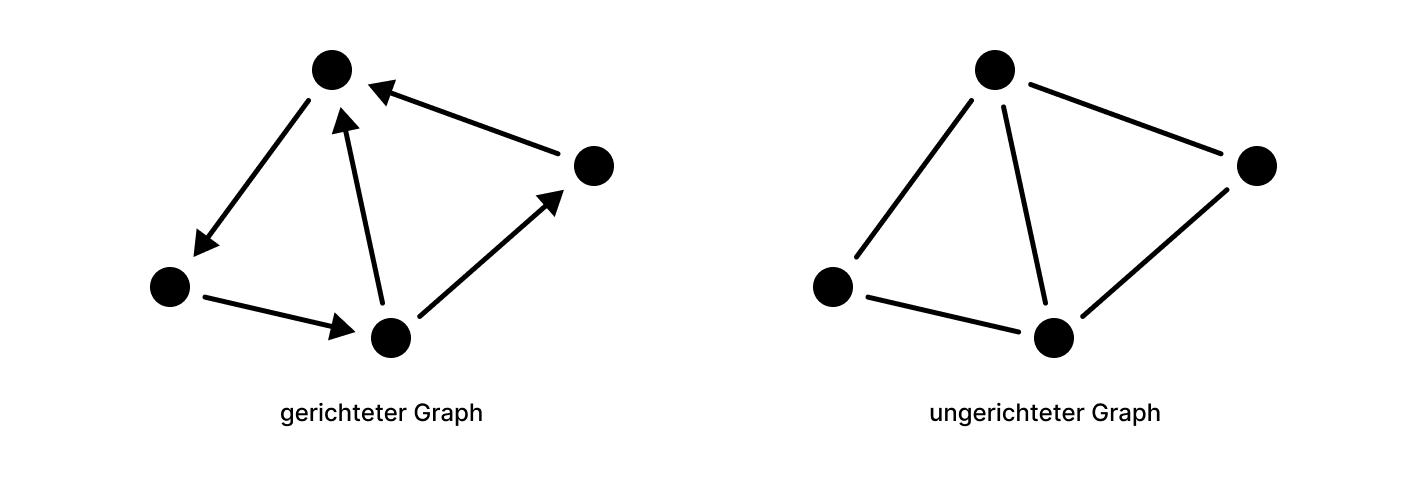
\includegraphics[width=1\textwidth]{content/img/Research/Graphen/Ausrichtung.png}
    \caption{Ein Graph mit gerichteten Kanten (links); ein Graph, dessen Kantenrichtung keine Bedeutung hat (rechts)}
    \label{fig:ausrichtung}
\end{figure}
\FloatBarrier